\documentclass[12pt]{article}
\usepackage{amsmath}
\usepackage{parskip}
\usepackage{setspace}
\usepackage{subfig}
\usepackage{fullpage}
\usepackage{tikz}
\usepackage{subcaption}
\usepackage{verbatim}
\usepackage{wrapfig}
\usepackage[margin=2cm]{geometry}

\begin{document}
$X_t$ follows the 
\[
\operatorname{SDE} \, dX = \mu(X, t) \, dt + e^Y \sigma(X, t) \, dW_t,
\]
and $Y_t$ follows an Ornstein-Uhlenbeck process
\[
dY = \kappa(\alpha - Y) \, dt + \Omega \, dW',
\]
with $dW \, dW' = \rho \, dt$.

The backward PDE reads:
\[
\partial_t V + e^{2y} \frac{\sigma(x, t)^2}{2} \partial_{xx}^2 V + e^y \sigma(x, t) \rho \Omega \partial_{xy}^2 V + \frac{\Omega^2}{2} \partial_{yy}^2 V + \mu(x, t) \partial_x V + \mu'(y, t) \partial_y V = 0.
\]

For the term involving the cross derivative, i.e., $\boxed{e^y \sigma(x, t) \rho \Omega \partial_{xy}^2 V}$,
\begin{itemize}
    \item If $\rho > 0$, the up-and-up in spot and vol, and the down-and-down in spot and vol are included. The corresponding cross matrix $\hat{L}$ is the same as in JJ's (cf. Eq (23)).
    \begin{center}
    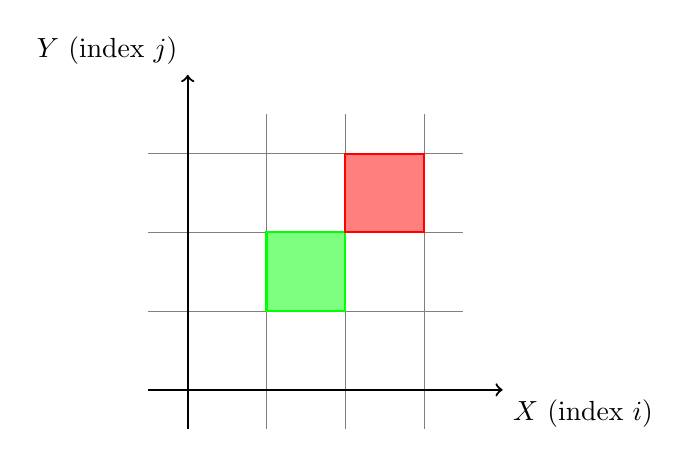
\begin{tikzpicture}
        % Draw the grid
        \draw[step=1cm,gray,very thin] (-0.5,-0.5) grid (3.5,3.5);    
        % Draw the axes
        \draw[thick,->] (-0.5,0) -- (4,0) node[anchor=north west] {$X$ (index $i$)};
        \draw[thick,->] (0,-0.5) -- (0,4) node[anchor=south east] {$Y$ (index $j$)};    
        % Draw the green square
        \filldraw[green, opacity=0.5] (1,1) rectangle (2,2);
        \draw[green, thick] (1,1) -- (2,1) -- (2,2) -- (1,2) -- cycle;    
        % Draw the red square
        \filldraw[red, opacity=0.5] (2,2) rectangle (3,3);
        \draw[red, thick] (2,2) -- (3,2) -- (3,3) -- (2,3) -- cycle;
    \end{tikzpicture}
    \end{center}    
    \begin{equation}
        \partial^2_{xy} V \approx \frac{1}{2 \Delta x \Delta y} \left( (V_{i+1, j+1} - V_{i, j+1}) - (V_{i+1, j} - V_{i, j}) + (V_{i, j} - V_{i-1, j}) - (V_{i, j-1} - V_{i-1, j-1}) \right)
    \end{equation}
    Let $q = -\frac{1}{2 \Delta x \Delta y} \rho \Omega$, we have
    \begin{equation}
        \rho \Omega \partial^2_{xy} V \approx q \left( (-V_{i+1, j+1} + V_{i, j+1}) + (V_{i+1, j} - 2V_{i, j} + V_{i-1, j}) + (V_{i, j-1} - V_{i-1, j-1}) \right).
    \end{equation}
    
    \item If $\rho < 0$, the up-and-down in spot and vol, and the down-and-up in spot and vol are included. The corresponding cross matrix $\hat{L}$ will be different from the positive $\rho$ case.
    \begin{center}
    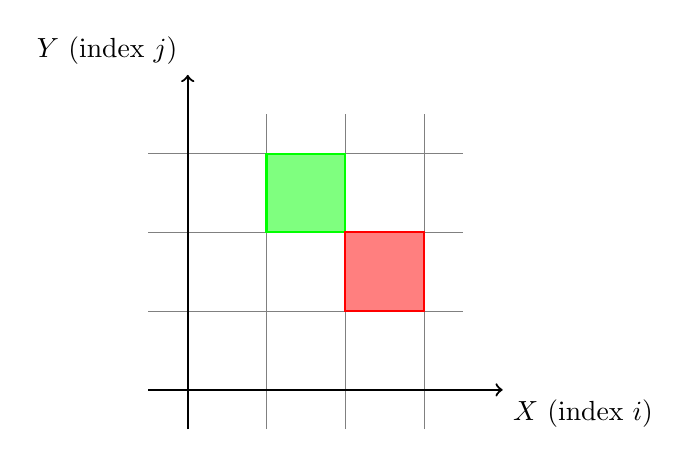
\begin{tikzpicture}    
        % Draw the grid
        \draw[step=1cm,gray,very thin] (-0.5,-0.5) grid (3.5,3.5);
        % Draw the axes
        \draw[thick,->] (-0.5,0) -- (4,0) node[anchor=north west] {$X$ (index $i$)};
        \draw[thick,->] (0,-0.5) -- (0,4) node[anchor=south east] {$Y$ (index $j$)};
        % Draw the green square
        \filldraw[green, opacity=0.5] (1,2) rectangle (2,3);
        \draw[green, thick] (1,2) -- (2,2) -- (2,3) -- (1,3) -- cycle;
        % Draw the red square
        \filldraw[red, opacity=0.5] (2,1) rectangle (3,2);
        \draw[red, thick] (2,1) -- (3,1) -- (3,2) -- (2,2) -- cycle;
    \end{tikzpicture}
    \end{center}        
    Similarly, let $q = -\frac{1}{2 \Delta x \Delta y} \rho \Omega$, we have
    \begin{equation}
        \rho \Omega \partial^2_{xy} V \approx q \left( (V_{i, j+1} - V_{i-1, j+1}) + (V_{i+1, j} - 2V_{i, j} + V_{i-1, j}) + (-V_{i+1, j-1} + V_{i, j-1}) \right).
    \end{equation}
    
    With the negative $\rho$, the cross matrix $\hat{L}$ is modified to
    \begin{equation}\label{eq: modified L_hat}
        \hat{L} = \left[\begin{array}{ccccc}L^{\prime} & Y & & & \\ Z & L'' & Y & & \\ & \cdots & \ldots & \cdots & \\ & & Z & L'' & Y \\ & & & Z & L^{\prime\prime} \end{array}\right],
    \end{equation}
    where the middle blocks are:
    
    \[
    L'' = \left[\begin{array}{cccccc}
    0 & 0 & & & & \\
    q & -2q & q & & & \\
    & q & -2q & q & & \\
    & & \cdots & \cdots & \cdots & \\
    & & & q & -2q & q \\
    & & & & 0 & 0
    \end{array}\right]
    \]
    
    \[
    Y = \left[\begin{array}{cccccc}
    0 & & & & & \\
    -q & q & & & & \\
    & -q & q & & & \\
    & & \cdots & \cdots & \cdots & \\
    & & & -q & q & \\
    & & & & & 0
    \end{array}\right]
    \]
    
    \[
    Z = \left[\begin{array}{cccccc}
    0 & & & & & \\
    & q & -q & & & \\
    & & q & -q & & \\
    & & \cdots & \cdots & \cdots & \\
    & & & & q & -q \\
    & & & & & 0
    \end{array}\right]
    \]

    The upper border is:

    \[
    L' = \left[\begin{array}{cccccc}
    0 & 0 & & & & \\
    q & -q & 0 & & & \\
    & q & -q & 0 & & \\
    & & \cdots & \cdots & \cdots & \\
    & & & q & -q & 0 \\
    & & & & 0 & 0
    \end{array}\right]
    \]

    The lower border is:

    \[
    L^{\prime\prime} = \left[\begin{array}{cccccc}
    0 & 0 & & & & \\
    0 & -q & q & & & \\
    & 0 & -q & q & & \\
    & & \cdots & \cdots & \cdots & \\
    & & & 0 & -q & q \\
    & & & & 0 & 0
    \end{array}\right]
    \]
    
    In other words, compared to Eq (23) in JJ's work, in the negative $\rho$ case, we flipped these matrices along the diagonal.
    
\end{itemize}
\vspace{0.5cm}

Below are eight graphs representing the transition matrix under flat local volatility. The four graphs in the left column correspond to the $\hat{L}$ matrix defined in JJ's work, with vol of vol ($\Omega$) set to $1 \times 10^{-4}$ and 0.75, and $\rho$ values of $\pm 0.75$. The right column consists of four graphs that apply the modified $\hat{L}$ matrix defined in \eqref{eq: modified L_hat}, using the same choices of vol of vol and $\rho$.

\begin{figure}[ht]
    \centering
    \begin{minipage}{0.45\textwidth}
        \centering
        \includegraphics[width=\textwidth]{fig/BEFORE_Density_plot_with_rho_0.75_omega_0.0001.jpg}
        \caption{[B] \(\Omega = 1 \times 10^{-4}\), \(\rho = 0.75\)}
    \end{minipage}
    \hfill
    \begin{minipage}{0.45\textwidth}
        \centering
        \includegraphics[width=\textwidth]{fig/AFTER_Density_plot_with_rho_0.75_omega_0.0001.jpg}
        \caption{[A] \(\Omega = 1 \times 10^{-4}\), \(\rho = 0.75\)}
    \end{minipage}

    \vspace{1em}

    \begin{minipage}{0.45\textwidth}
        \centering
        \includegraphics[width=\textwidth]{fig/BEFORE_Density_plot_with_rho_-0.75_omega_0.0001.jpg}
        \caption{[B] \(\Omega = 1 \times 10^{-4}\), \(\rho = -0.75\)}
    \end{minipage}
    \hfill
    \begin{minipage}{0.45\textwidth}
        \centering
        \includegraphics[width=\textwidth]{fig/AFTER_Density_plot_with_rho_-0.75_omega_0.0001.jpg}
        \caption{[A] \(\Omega = 1 \times 10^{-4}\), \(\rho = -0.75\)}
    \end{minipage}

    \vspace{1em}

    \begin{minipage}{0.45\textwidth}
        \centering
        \includegraphics[width=\textwidth]{fig/BEFORE_Density_plot_with_rho_0.75_omega_0.75.jpg}
        \caption{[B] \(\Omega = 0.75\), \(\rho = 0.75\)} \label{fig: before change, 0.75 omega and 0.75 rho}
    \end{minipage}
    \hfill
    \begin{minipage}{0.45\textwidth}
        \centering
        \includegraphics[width=\textwidth]{fig/AFTER_Density_plot_with_rho_0.75_omega_0.75.jpg} 
        \caption{[A] \(\Omega = 0.75\), \(\rho = 0.75\)} \label{fig: after change, 0.75 omega and 0.75 rho}
    \end{minipage}

    \vspace{1em}

    \begin{minipage}{0.45\textwidth}
        \centering
        \includegraphics[width=\textwidth]{fig/BEFORE_Density_plot_with_rho_-0.75_omega_0.75.jpg}
        \caption{[B] \(\Omega = 0.75\), \(\rho = -0.75\)} \label{fig: before change, 0.75 omega and -0.75 rho}
    \end{minipage}
    \hfill
    \begin{minipage}{0.45\textwidth}
        \centering
        \includegraphics[width=\textwidth]{fig/AFTER_Density_plot_with_rho_-0.75_omega_0.75.jpg}
        \caption{[A] \(\Omega = 0.75\), \(\rho = -0.75\)} \label{fig: after change, 0.75 omega and -0.75 rho}
    \end{minipage}
\end{figure}

With the correctly identified cross matrix \(\hat{L}\), the transition density appears symmetric for both negative (Fig. \ref{fig: after change, 0.75 omega and -0.75 rho}) and positive (Fig. \ref{fig: before change, 0.75 omega and 0.75 rho}) \(\rho\) cases under the flat LV tests. However, when an incorrectly identified cross matrix is applied, the transition density seems to exhibit skewness in both cases (positive \(\rho\): Fig. \ref{fig: after change, 0.75 omega and 0.75 rho} and negative \(\rho\): Fig. \ref{fig: before change, 0.75 omega and -0.75 rho}).

\end{document}
